\documentclass[lettersize,journal]{IEEEtran}
\usepackage{amsmath,amsfonts}
\usepackage{algorithmic}
\usepackage{algorithm}
\usepackage{array}
\usepackage[caption=false,font=normalsize,labelfont=sf,textfont=sf]{subfig}
\usepackage{textcomp}
\usepackage{stfloats}
\usepackage{url}
\usepackage{verbatim}
\usepackage{graphicx}

\hyphenation{op-tical net-works semi-conduc-tor IEEE-Xplore}

\begin{document}

\title{OUXT Polaris: Autonomous Navigation System for the 2022 Maritime RobotX Challenge}
\author{
    Kenta Okamoto,Kyoto Institute of Tech., m2623106@edu.kit.ac.jp \\ \and
    Akihisa Nagata, Kansai Univ. , k065604@kansai-u.ac.jp \\ \and
    Kyoma Arai, Tokai Univ. , 2cemm007@mail.u-tokai.ac.jp \\ \and
    Masato Kobayashi, Kobe Univ. , 171w951w@gsuite.kobe-u.ac.jp \\ \and
    Yusei Nagao, Osaka Institute of Tech., m1m22r23@oit.ac.jp \\ \and
    Tatsuki Nishimura, Osaka Univ., hbvcg00@gmail.com \\ \and
    Shunya Tanaka, , syun111@gmail.com \\ \and
    Masaya Kataoka, TIER IV inc . , ms.kataoka@gmail.com,
}

% The paper headers
\markboth{Maritime RobotX Challenge 2022}%
{Shell \MakeLowercase{\textit{et al.}}: A Sample Article Using IEEEtran.cls for IEEE Journals}

% \IEEEpubid{0000-0000/00\$00.00~\copyright~2021 IEEE}
% Remember, if you use this you must call \IEEEpubidadjcol in the second
% column for its text to clear the IEEEpubid mark.

\maketitle

\begin{abstract}
OUXT-Polaris has been developing an autonomous navigation system by participating in the 
Maritime RobotX Challenge 2014, 2016, and 2018. 
In this paper, we describe the improvement of the previous vessel system. 
We also indicate the advantage of the improved design.
Moreover, we describe the developing method for Covid-19 and the 
feature components for the next RobotX Challenge.
\end{abstract}

\begin{IEEEkeywords}
Maritime systems, Robotics, Unmanned surface vehicle
\end{IEEEkeywords}

\section{Introduction}
First of all, we are motivated to develop a big field robot in a large area such as the ocean.
In recent years, the aging and shrinking population, as well as a shortage of workers,
has led to an increase in demand for the automation of cars, robots, and other equipment.
Among these, automated driving is being developed with particular emphasis.
Moving the autonomous vehicle or robot outside has a very severe problem.
They need to hedge unknown obstacles and go to the target position.
The environment such as weather, temperature, or underwater around robots causes sensor and hardware problems.
There are each challenging problems and They are also interesting for us, and there are different problems between land and ocean.
On the land, the navigation or the estimation of the self-position is solved by the point cloud map and the odmetry,
while on the ocean, the point cloud and the odmetry is not obtained enough. So the robots need to estimate the self-position using GPS and IMU sensors.
Moreover, on the land, the position of the target objects and obstacles is obtained from Lidar data. On the other hand in the sea,
waves disturbe to get the target positions. In that case, the robots have to fusion multiple data such as cameras and Lidars.
In this competition, we have a chance to develop a system to get over the wild environment 
for the robots on the ocean. Therefore, we are participating in the Maritime RobotX Challenge.

\section{Overview of vessel system}
First, we describe the architecture of the navigation system. As you can see Fig. \ref{fig:arch_nav},
the position and the velocity of WAM-V are estimated using the 6DoF Extended Kalman Filter \cite{robotx_ekf}
from the data of the GNSS and IMU sensors.
The obstacles and task objects are recognized from lidar and camera data. Based on the self-position and the task objects, 
WAM-V decides where to go and what to do next.
After getting the target position, the path is created by the path planner,
and the target velocity that WAM-V can trace the way is calculated. 
Finally, in the servo and thruster controllers,
the servo motor direction and the thruster revolution to achieve the target velocity are calculated based on the vessel motion model.

\begin{figure}[htbp]
    \begin{center}
        \scalebox{0.8}{
            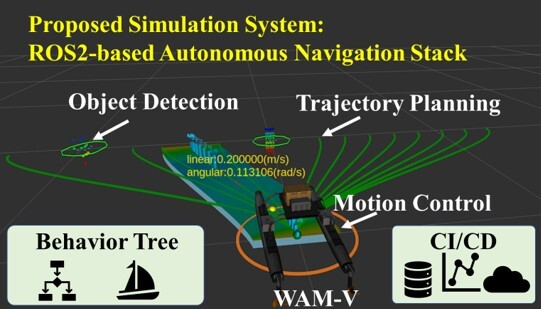
\includegraphics{figure/proposed_sw_system.jpg}
        }
    \end{center}
    \caption{the archtecture of navigation system}
    \label{fig:arch_nav}
\end{figure}

\section{Hardware Developments}

\subsection{Redesign of Azimuth Thruster}

We considered the following three issues when designing the propulsion mechanism.

First, we considered it important for the boat to be able to generate lateral propulsive force to complete the docking task.
When propulsion units are mounted on the two aft sections of the boat, each propulsion unit must have a degree of freedom in the yaw axis to generate thrust in any direction in the horizontal plane.
This propulsion system is generally called an azimuth thruster.

Next, the electric outboard motors that are commonly available have a circular cross-section for the mounting shaft, so it is necessary to find a way to fix the shaft tightly.

In addition, the propeller must avoid contact with the seafloor when the vessel needs to navigate in shallow water, such as when launching the boat on the course. Since it is dangerous for a person to enter shallow water and lift the thruster with a tool, a mechanism that can easily raise and lower the thruster was necessary.

To meet these requirements, we designed the mechanism shown in Fig. \ref{fig:azimuth_design}.
The three functions of gripping, rotating, and elevating are integrated into a single unit.

The gripping function was realized using a PLA plastic collet manufactured by a 3D printer.
The collet is pushed axially by a screw into an aluminum hollow shaft with a wedge-shaped cross section to enable strong shaft gripping.

The azimuth mechanism is realized by transmitting the rotational force from the servo motor (XM540-W270, Dynamixel) to the hollow shaft by spur gears.
The hollow shaft is held at two points by angular bearings.

\begin{figure}[htbp]
  \begin{center}
    \scalebox{0.2}{
      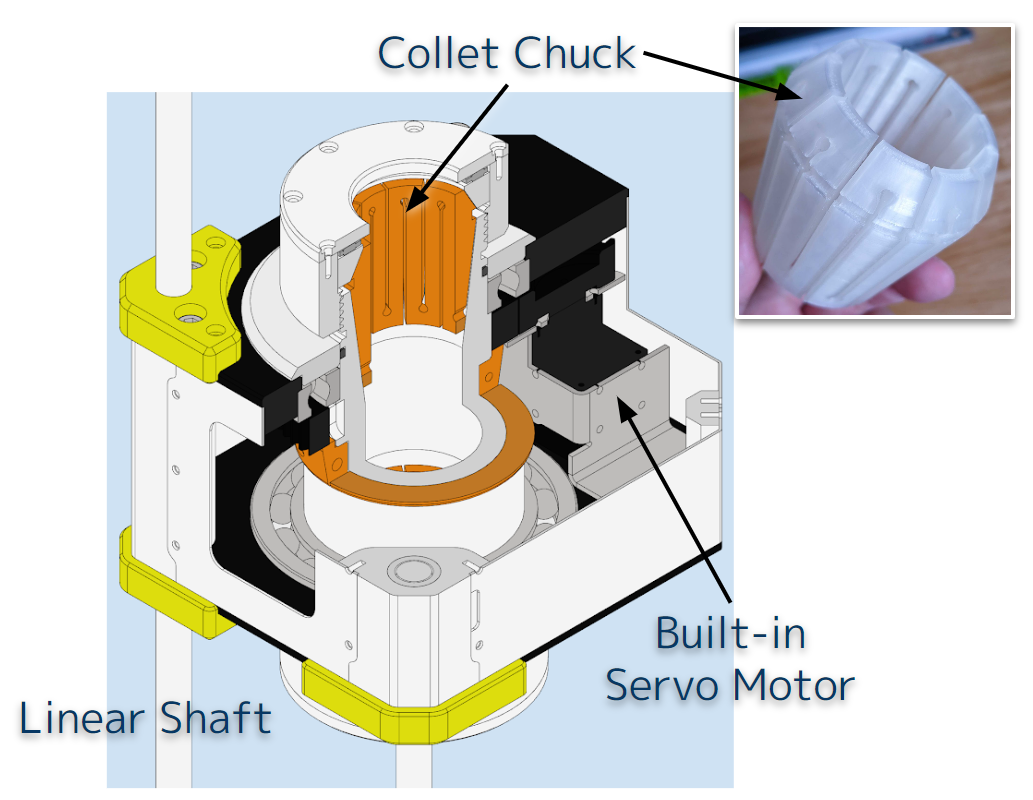
\includegraphics{figure/azimuth_thruster.png}
    }
  \end{center}
  \caption{The design of azimuth thruster}
  \label{fig:azimuth_design}
\end{figure}


\subsection{MINI-V in the COVID-19}
MINI-V(minitua vessel) was created in order to test the software easily in the Covid-19. Over the past several years, 
we couldn't conduct the experiment on the ocean or lake because of the COVID-19.
We were prohibited to meet and create the parts of WAM-V.
In addition, the law about vessels is very strict.
So, we can't float the boat easily. The WAM-V is so big and it is hard work and costs too much to carry WAM-V to the lake. 
Then, we need a sustainable system to develop the automotive vessel.
As mentioned above, the simulator is used for developing navigation systems, and it doesn't need to use WAM-V.
The perception array was created to get the sensor data for software tests. They made it easier for us to develop software without ships.
However, the software and hardware integration is the most important to conduct tasks. Then, MINI-V was created 
to make it easier to do the test and the integration.

The concepts of MINI-V are follows:
\begin{enumerate}
  \item easy assembly, transport, and experiment,
  \item open source software and hardware,
  \item high compatibility between WAM-V and MINI-V.
\end{enumerate}

\begin{figure}[htbp]
  \begin{center}
    \scalebox{0.2}{
      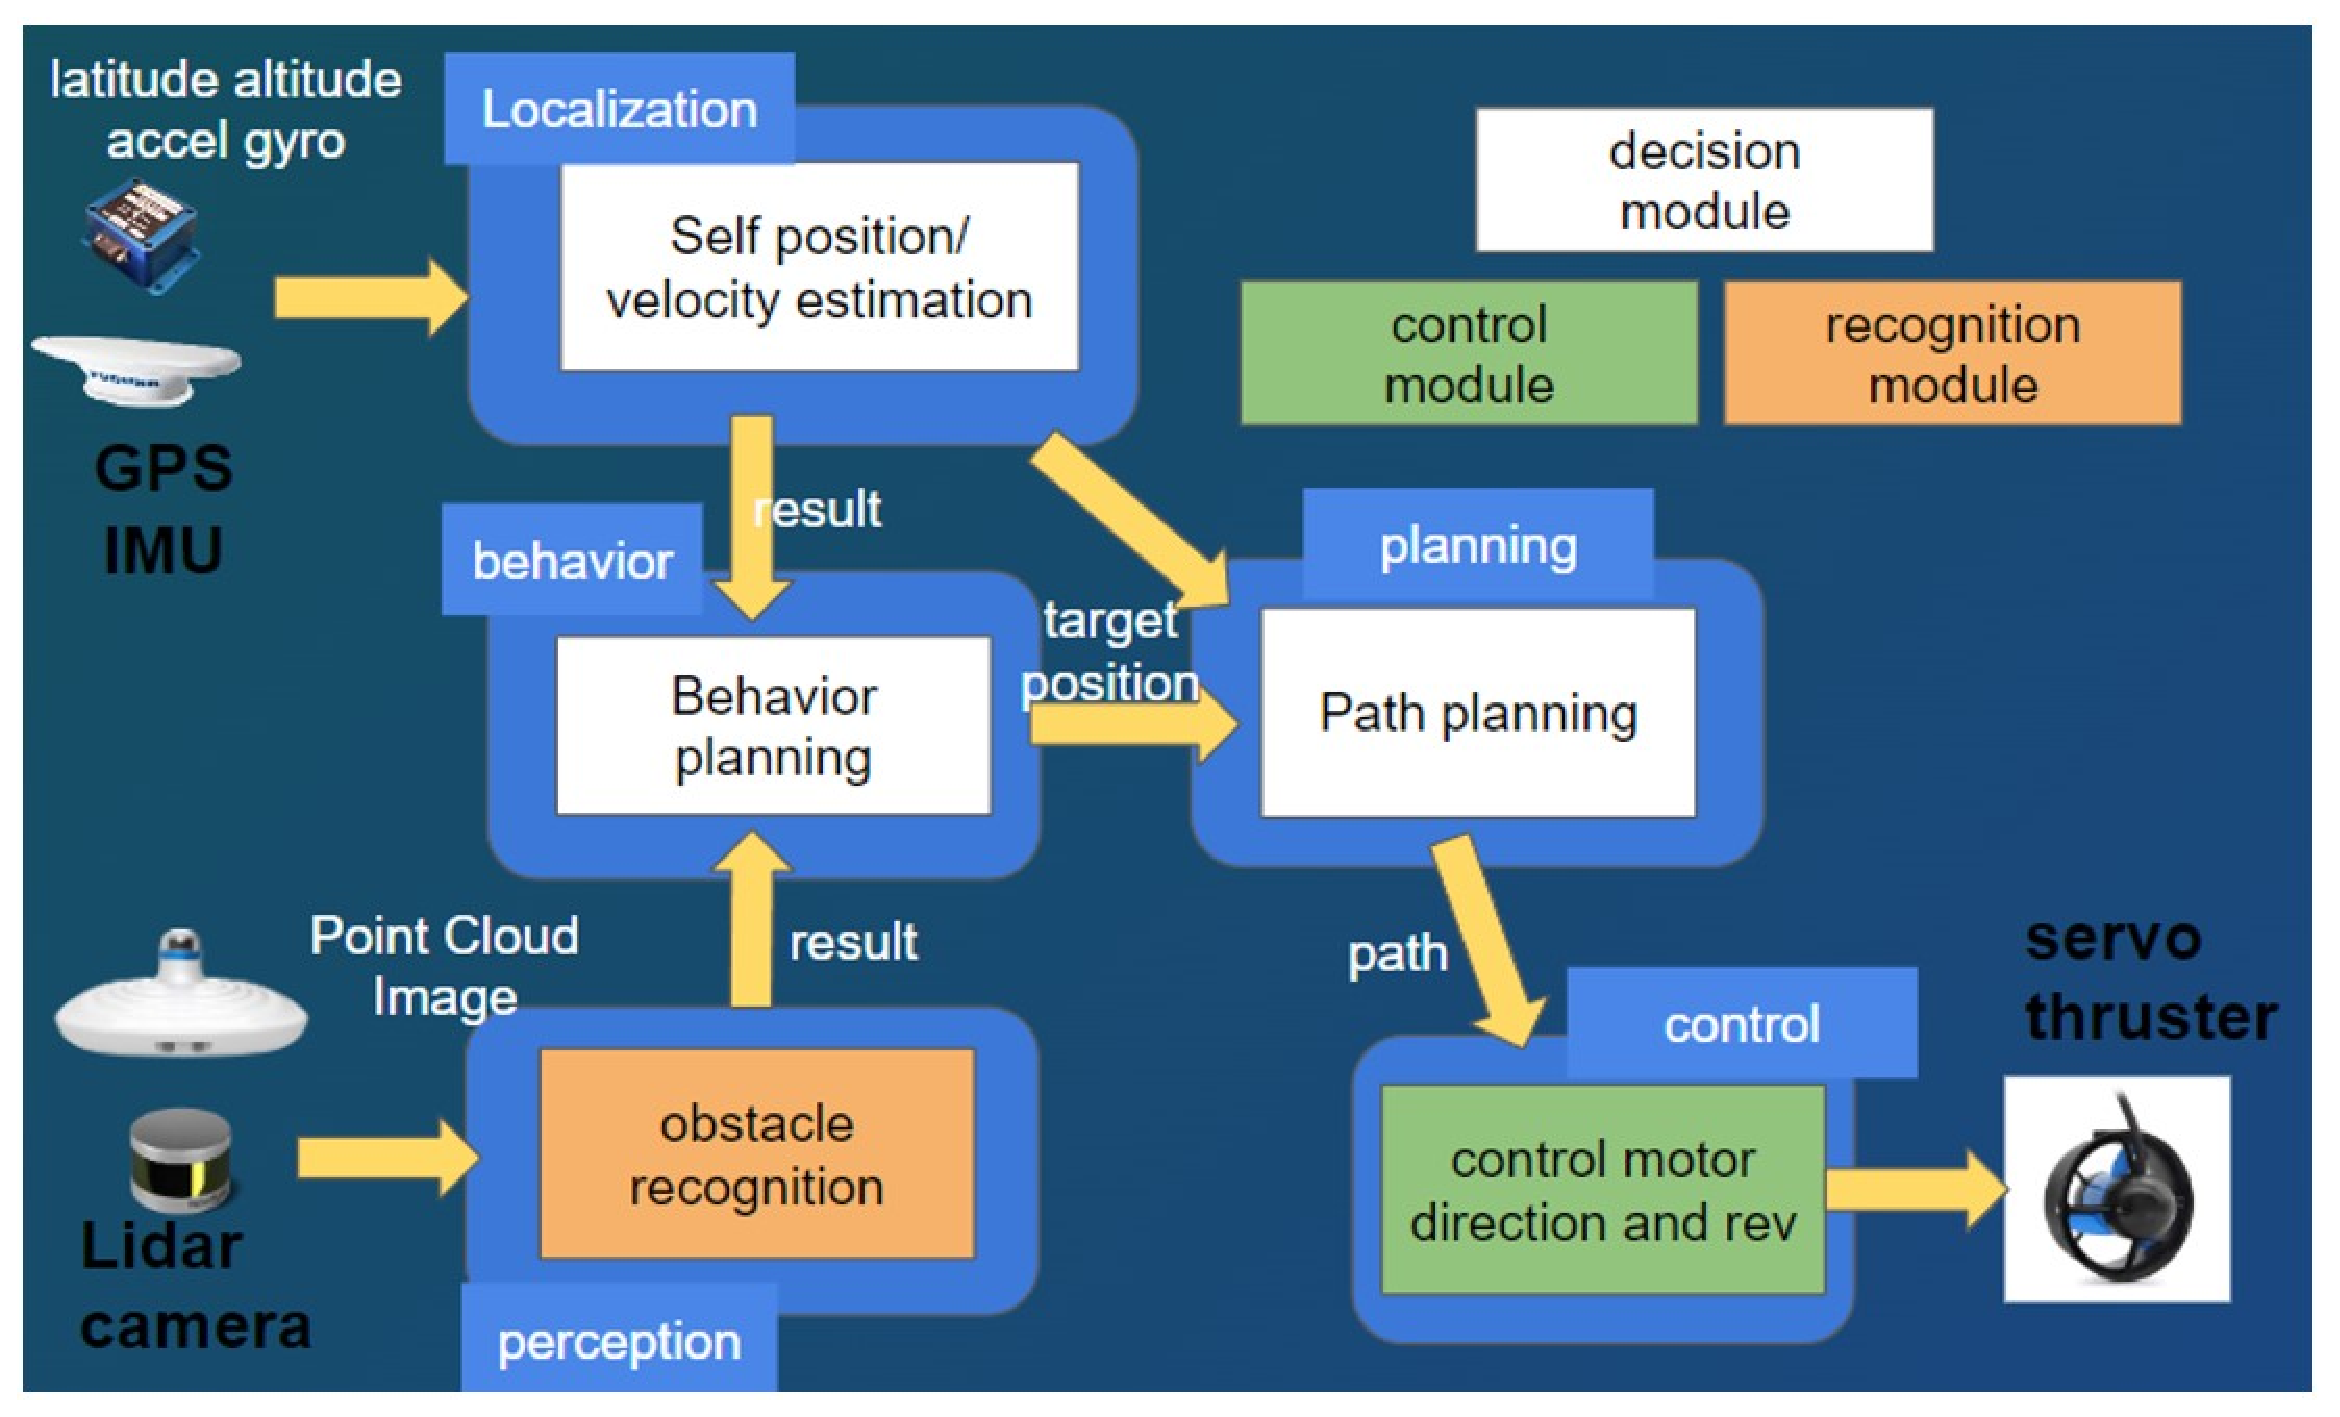
\includegraphics{figure/arch_nav.eps}
    }
  \end{center}
  \caption{the archtecture of navigation system}
  \label{fig:arch_nav}
\end{figure}

\begin{figure}[htbp]
    \begin{center}
      \scalebox{0.18}{
      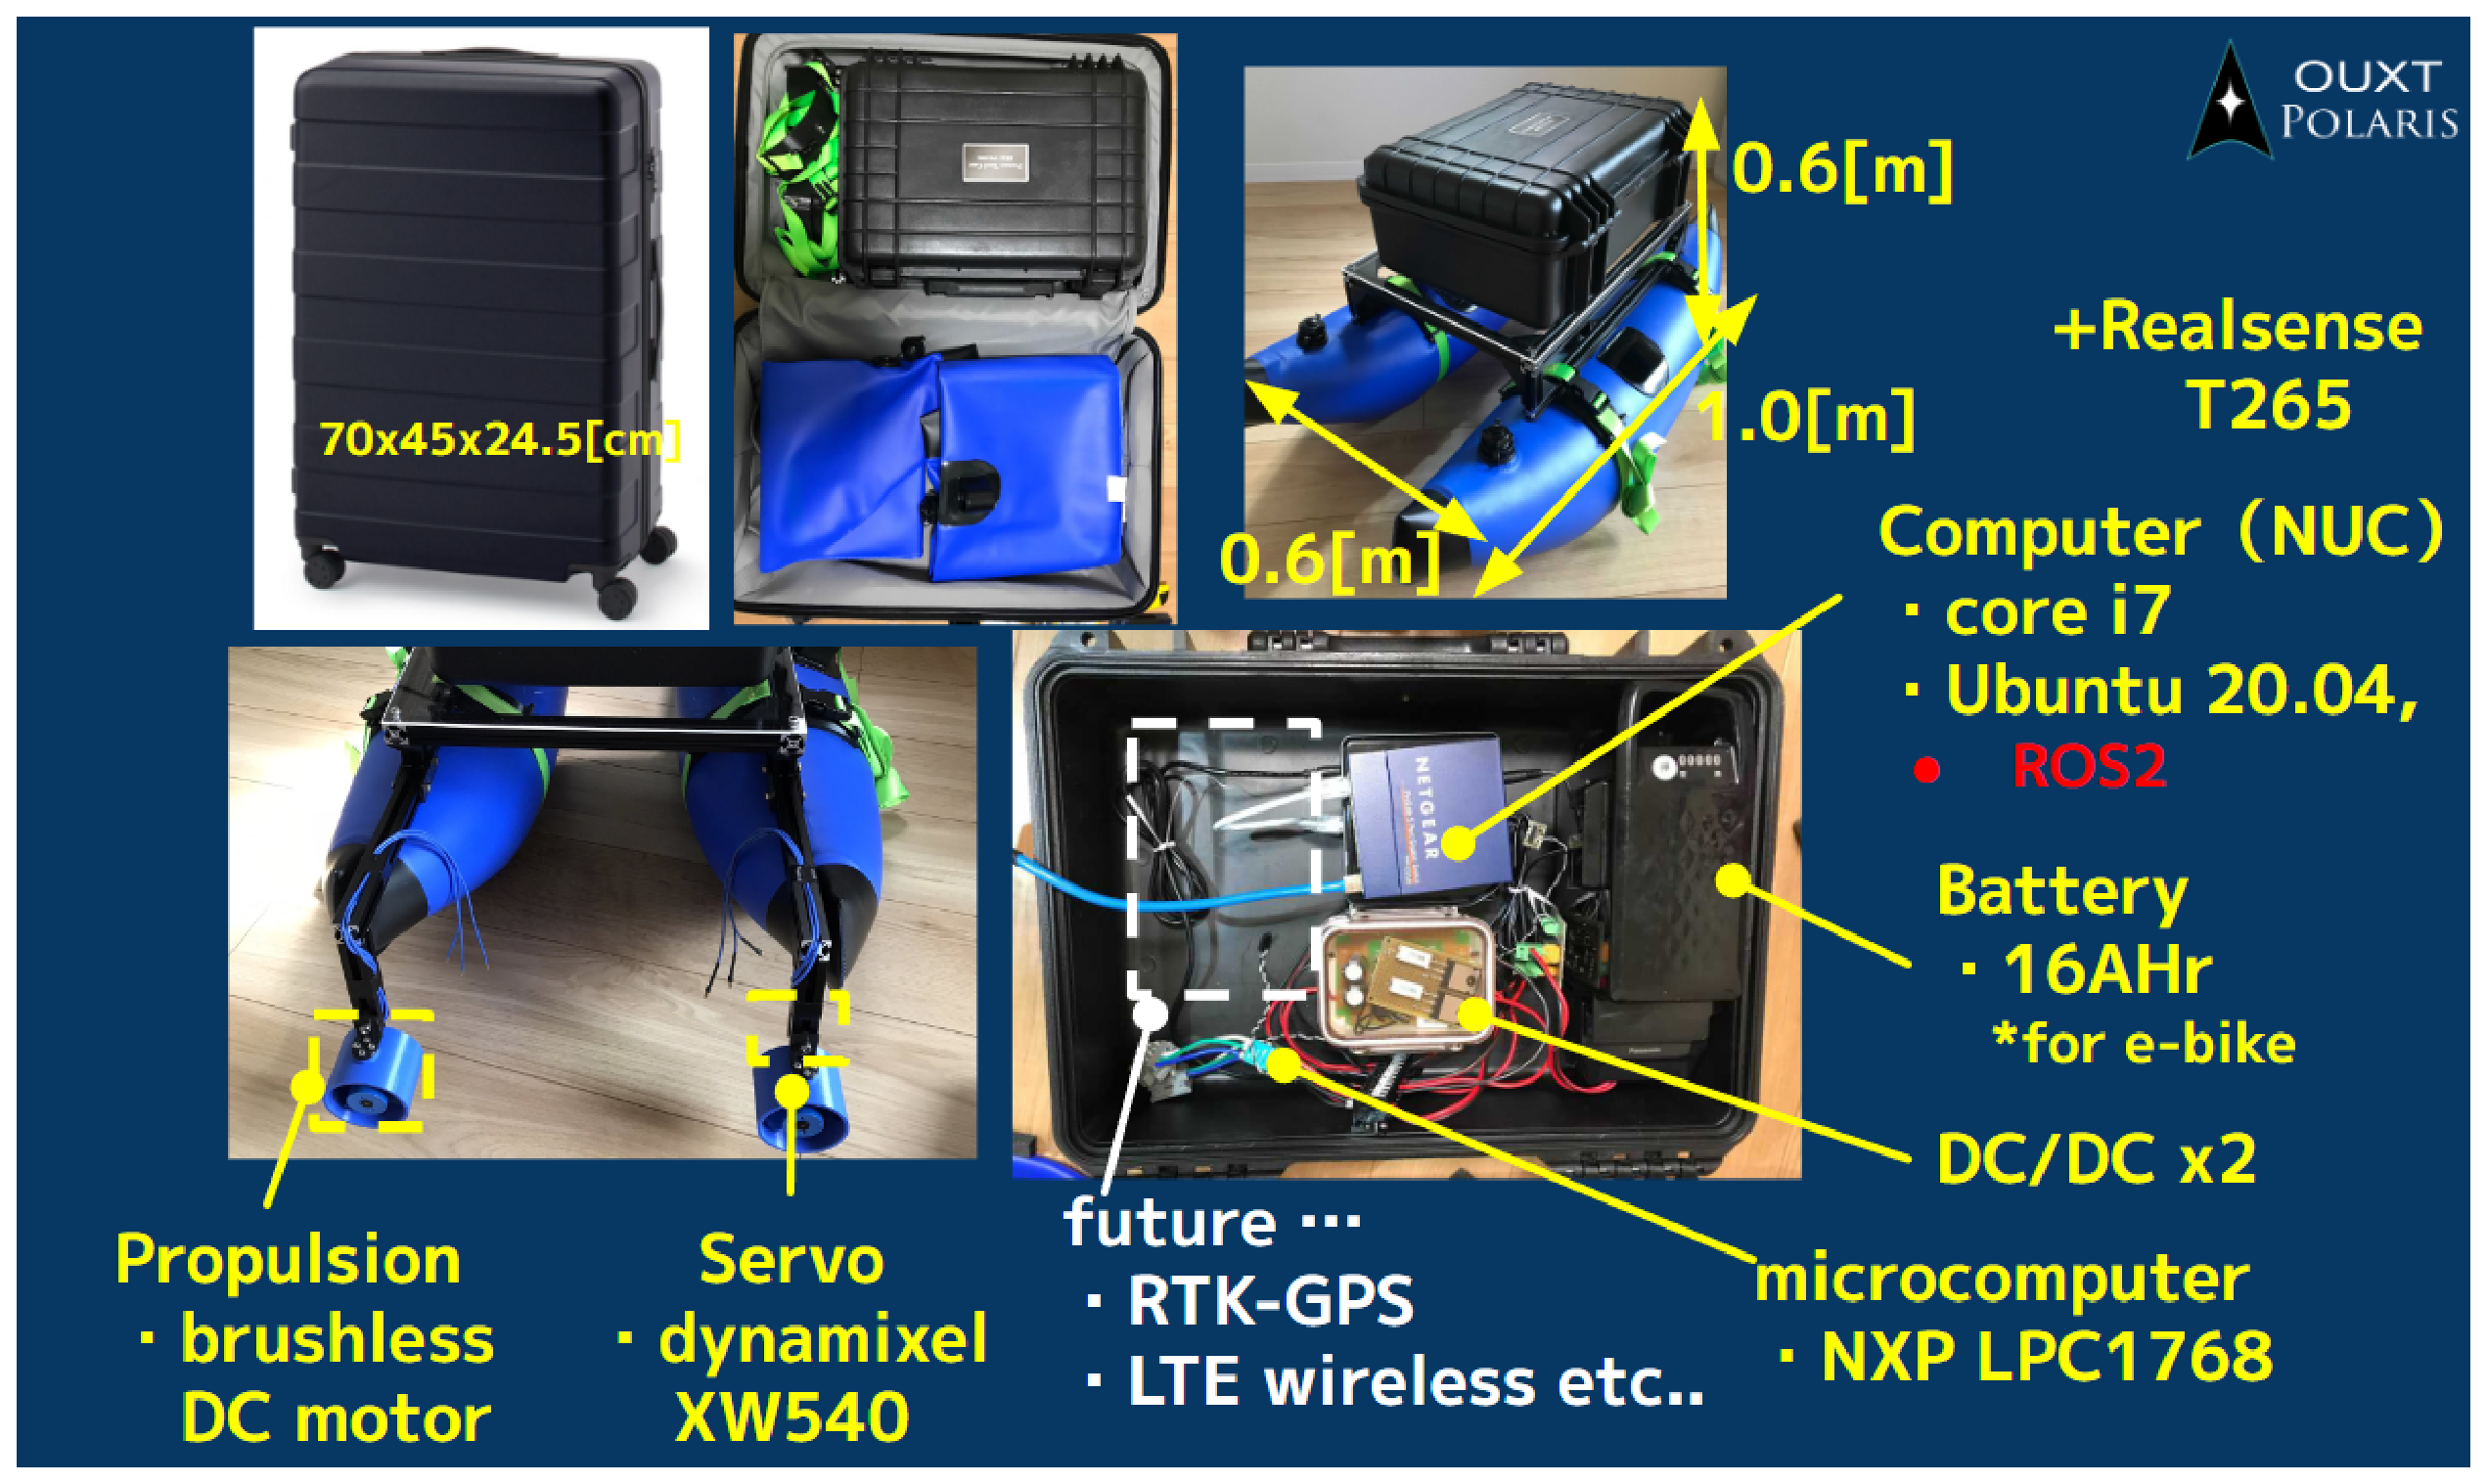
\includegraphics{figure/mini_v_component.eps}
    }
  \end{center}
  \caption{Hardware components of MINI-V}
  \label{fig:mini_v_component}
\end{figure}

\begin{figure}[htbp]
    \begin{center}
      \scalebox{0.28}{
        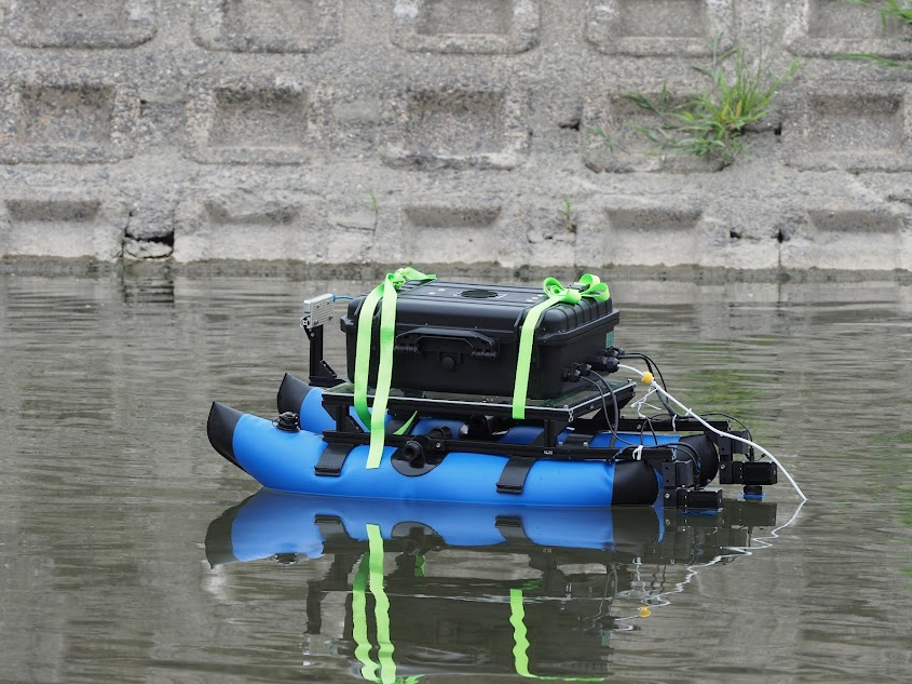
\includegraphics{figure/mini_v_overview.png}
      }
    \end{center}
    \caption{Experiment on the Ai river}
    \label{fig:mini_v_experiment}
  \end{figure}

MINI-V is created to be easy to carry, and we can carry them by suitcase like Fig. \ref{fig:mini_v_component}. It is so small that we can
float and test on the buthtab.
It is also assembled simply. We develop this vessel on open source. So, other people can play or test their software with MINI-V. Finally,
we expect the high compatibility between WAM-V and MINI-V, and it will make it easy to migrate developed software on MINI-V toWAM-V. However, 
MINI-V have not had complete compatibility yet.
We have future tasks to create a little bigger vessel to have compatible hardware and software such as batteries and sensors, and so on.

\subsection{the prototype of the multicopter}
In the RobotX 2022, the tasks about multicopter are add on the competition. The drone needs to be automated and pick up the task objects.
We created the quadcopter below in Fig.\ref{fig:drone}.
The flight controller, Pixacer Pro, is introduced to controll the drone. 
In order to get the drone position, it has GNSS sensor on the plane.
we conduct the test of estimating the self-position of the drone. As you can see Fig.\ref{fig:drone_posi} the drone can estimate
the self-position With an error of $\pm 0.5 \mathrm{m}$ approxmately.
At the moment. the drone is manually controled by a pilot but not automated.
For automation, we need to add computers such as raspberryPi to send the operation into flight controller. 
Moreover, the sensor such as cameras to recognize the task objects are needed.
There are many considerations such as the roter-size, motor power, the size of body, and so on.
We are going to develop the automated navigation system for drone in next years.

\begin{figure}[htbp]
  \begin{center}
    \scalebox{0.2}{
      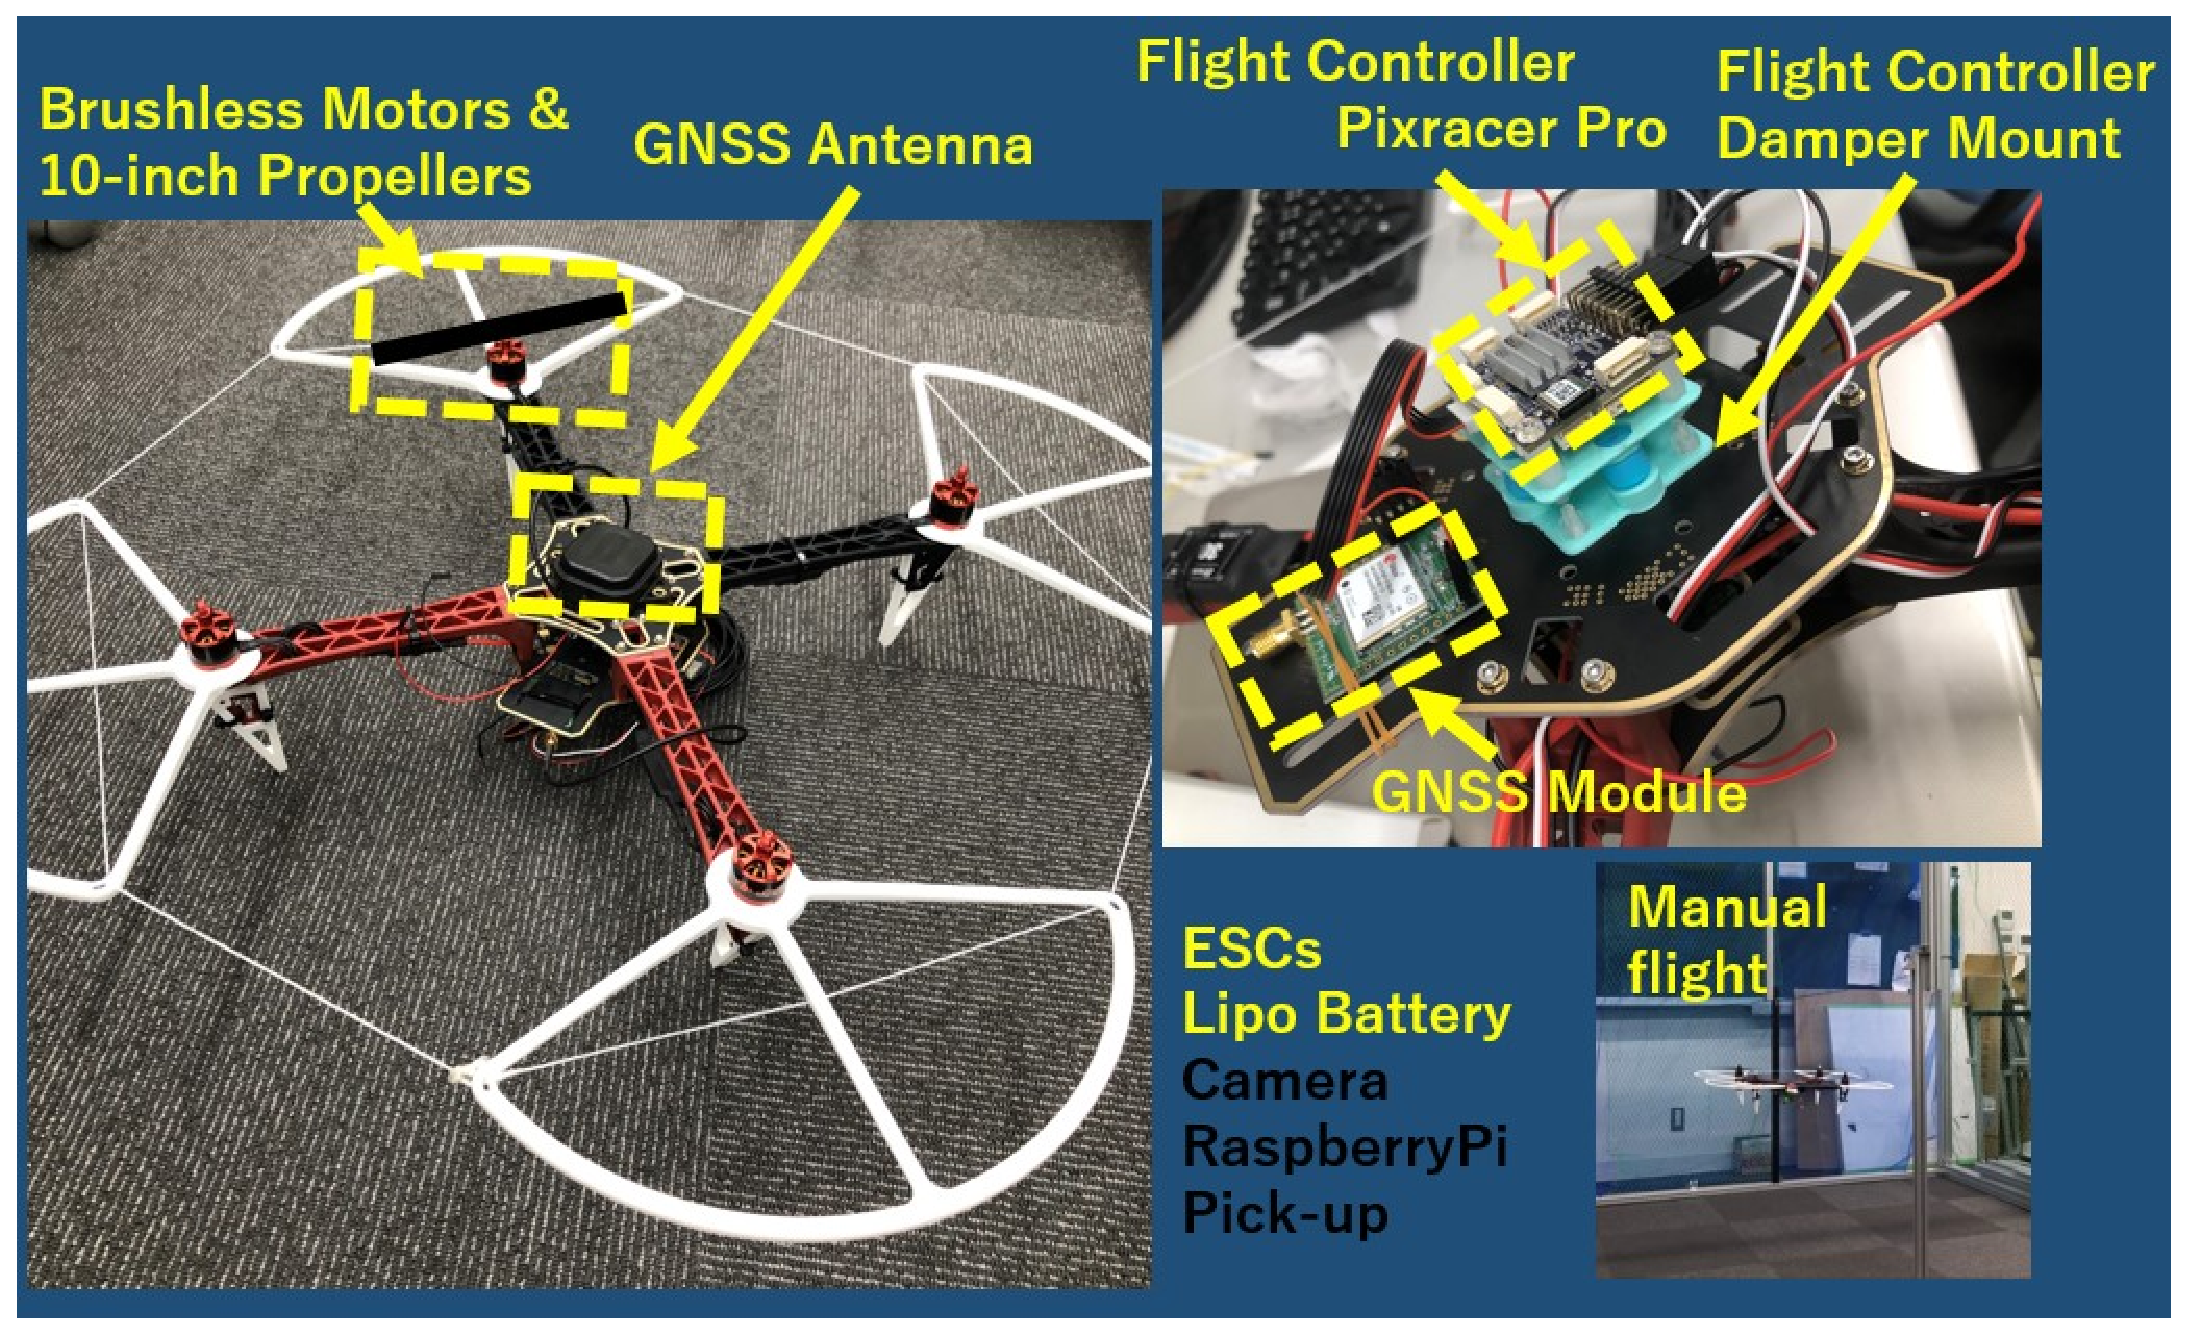
\includegraphics{figure/drone.eps}
    }
  \end{center}
  \caption{the componets of the drone}
  \label{fig:drone}
\end{figure}

\begin{figure}[htbp]
  \begin{center}
    \scalebox{0.4}{
      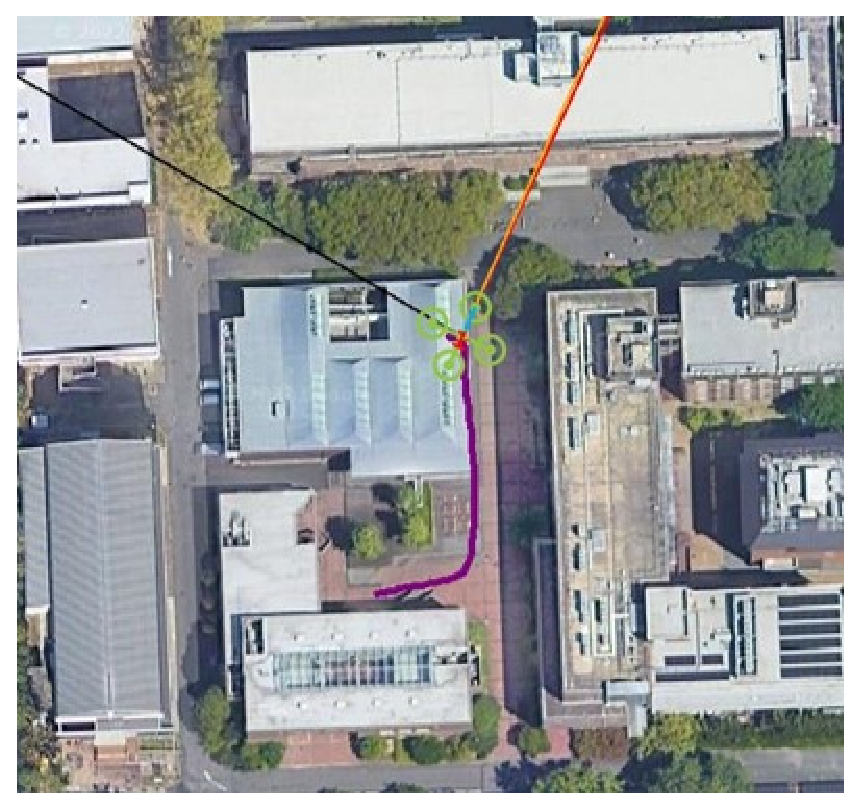
\includegraphics{figure/drone_posi.eps}
    }
  \end{center}
  \caption{the estimated drone position and the track}
  \label{fig:drone_posi}
\end{figure}


\section{Software Developments}
\subsection{ROS2-based Autonomous Navigation Stack}
In “Maritime RobotX Challenge 2018”, we used Robot Operating System 1(ROS1) for developing software.
However, the development of ROS1 was finished with python2 end of life.
Therefore, we adopted the next generation of ROS called “ROS2”. \cite{ROS2_paper}
As shown in Fig. 1, our ROS2-based simulation and software system was already developed.
Our software contributions are listed as follows.

\begin{itemize}
  \item {\it Software System }:
    We rebuilt the software system from ROS1 to ROS2
  \item {\it Behavior Tree}:
  We adopted the behavior tree library in ROS2 and built our original behavior tree.  
  \item {\it Camera LiDAR fusion}:
    We are developing a lidar-camera fusion object detection system for this project.
  \item {\it Simulation Tool Development }:
    We developed LiDAR simulation by using intel ray-tracing OSS "Embree".
  \item {\it Infrastructure}
    We developed some automation tools for develop quickly.
\end{itemize}
We published all codes in GitHub to give feedback knowledge to the ROS community and 
Open-Source all our resources not only software \cite{documentation_software}
but also CAD models, and circuit data. \cite{documentation_hardware}

\subsection{Software System Architecture}
Our navigation stack is based on ROS2, but we do not use the navigation2 library. We develop our original software.
Our software is highly modularized, so some of our members use our stacks in other autonomous mobility competitions.
All of our software is managed by ansible and can be deployed on real machines without the need for human intervention.
It is open source, including the setup tools \cite{ouxt_automation} and it's documentation \cite{documentation_software},
so anyone in the world can try out the OUXT-Polaris navigation stack.


\subsection{Camera LiDAR fusion}
We used YOLOX\cite{YOLOX} for object Detection of task object information such as buoys and docks.

\subsection{Behavior Tree}
Using behavior tree can build WAM-V behaviors like a tree.  
we used Groot for smooth development using behavior tree.

\begin{figure}[htbp]
  \begin{center}
    \scalebox{0.24}{
      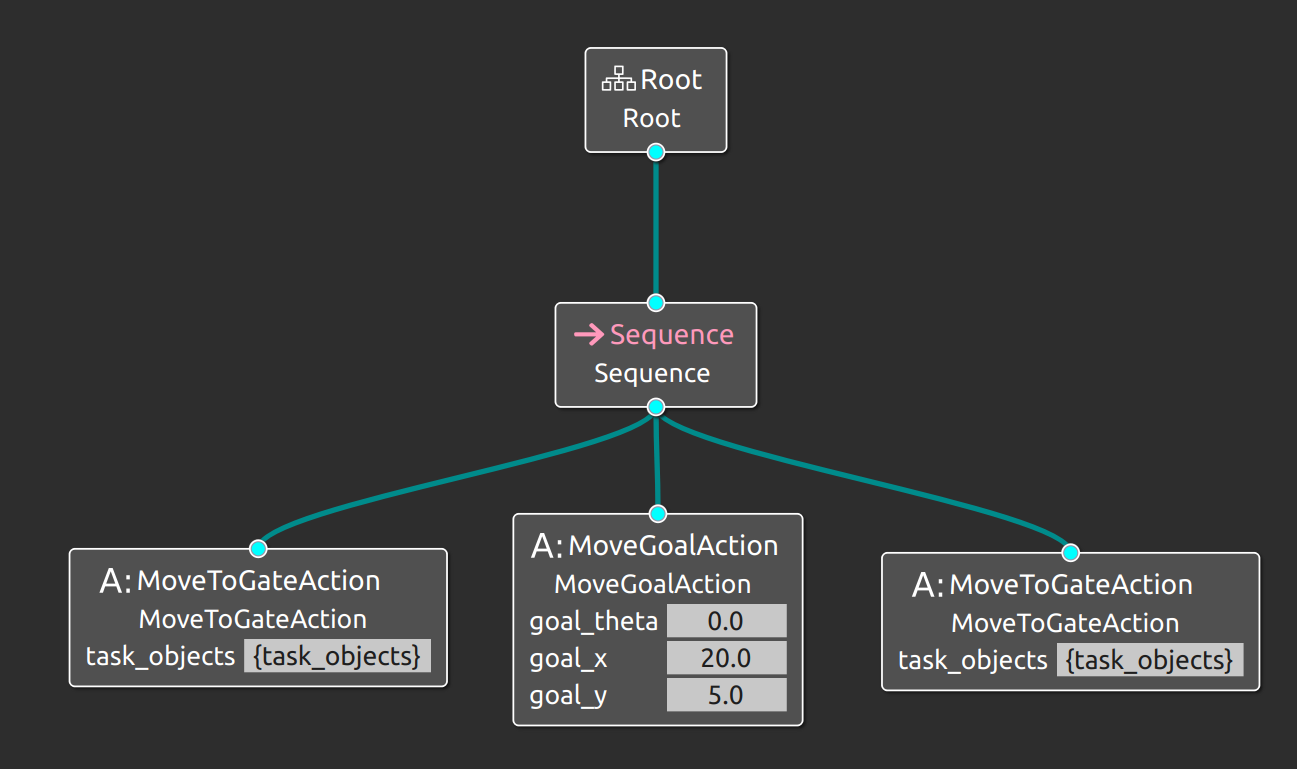
\includegraphics{figure/groot.png}
    }
  \end{center}
  \caption{Groot example}
  \label{fig:Groot}
\end{figure}

For example, in the WAM-V Dynamic Qualifying Task, 
we defined a node that navigation and searches channel markers.
In searching channel markers behavior, first, we got the information from the result of lidar-camera fusion object detection system. 
Information we can get from the system is objects label, probabilities, and bounding boxes.
And we convert the information we can get from the system into information containing channel markers information 
we can use in robotx challenge contains such as labels and distance from WAM-V etc.
After search channel markers, WAM-V starts navigation.
We need to act the Node two times in the task. So we defined two same nodes and connected them by Sequence node. 
The sequence node is defined in the behavior tree.
We made other Nodes, for example, move forward node, stop node and rotate around the buoy node.
These nodes can realize many behavior patterns required in tasks.

\subsection{Object Detection}
We used  YOLOX\cite{YOLOX} for object Detection of task object information such as buoys and docks.
We created annotation data based on images and videos obtained from past RobotX Challenges.
We open our annotation data for speeding up future development for Maritime RobotX. \cite{dataset_annotations}
The result of training and inference is shown in Fig. hoge. 
The image is part of a video recorded during our challenging navigation in the 2018 RobotX Challenge.\cite{RobotX2018_video}
\indent The point cloud from LiDAR preprocesses before fusion the camera image and the LiDAR point cloud.
First, The point cloud from the LiDAR is filtered to remove outliers.
Next, the filtered point cloud is downsampled to a 2D Laser Scan.
Then, the object area is extracted from the 2D LaserScan. \cite{scan_segmentation}
The extraction algorithm determines the object area information based on whether the distance between 
the neighboring LaserScan is less than the threshold value determined adaptively.
The clustered point cloud is projected on the camera images.
And we will match the bounding IOU and the object label on the images by Hungarian method.

\subsection{Infrastructure}
Our system runs in a complex distributed computing environment that includes microcontrollers,
so the configuration file is huge and there are many processes that need to be launched to start the system.
If such a system is deployed manually, various human errors are expected to occur.
In addition, there are 77 ROS2 packages that make up our autonomous navigation system,
and it is almost impossible to manage all of them manually without error.
To solve these problems, we used a configuration management tool called ansible.
ansible can support environment construction procedures on the computer in YAML format and
can switch between development and production environments with a single option.
With the adoption of ansible, setting up our system is just a matter of running a single shell script.

Also, even if the ROS2 package does not have any changes in the code of the package itself,
the software may break if there are changes in the packages on which the package depends.
To detect and fix this quickly, we built a CI system using GitHub Actions.
CI is a technology called continuous integration, which detects commits to Github, etc.,
and automatically performs tests to find defects early.
When a pull request is issued for any of the packages we manage, a build test is automatically performed once a day.
If the build test fails, the pull request cannot be merged.
Failed build tests are notified to the OUXT-Polaris Slack so that members know immediately if a failure has occurred.
Whole architecture of CI/CD pipeline shown in Fig.\ref{fig:ci_cd_pipeline}.

\begin{figure}[htbp]
    \begin{center}
      \scalebox{0.18}{
      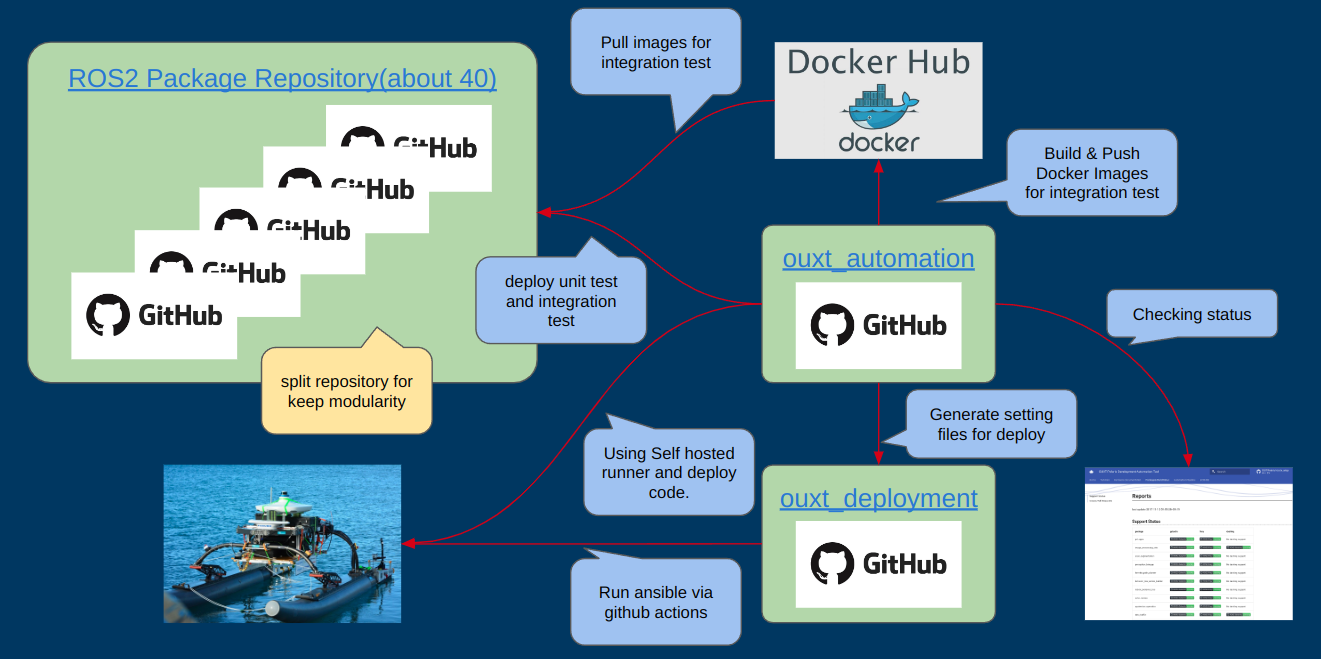
\includegraphics{figure/ci_cd_pipeline.png}
    }
  \end{center}
  \caption{CI/CD Pipeline}
  \label{fig:ci_cd_pipeline}
\end{figure}

\begin{figure}[htbp]
    \begin{center}
      \scalebox{0.18}{
      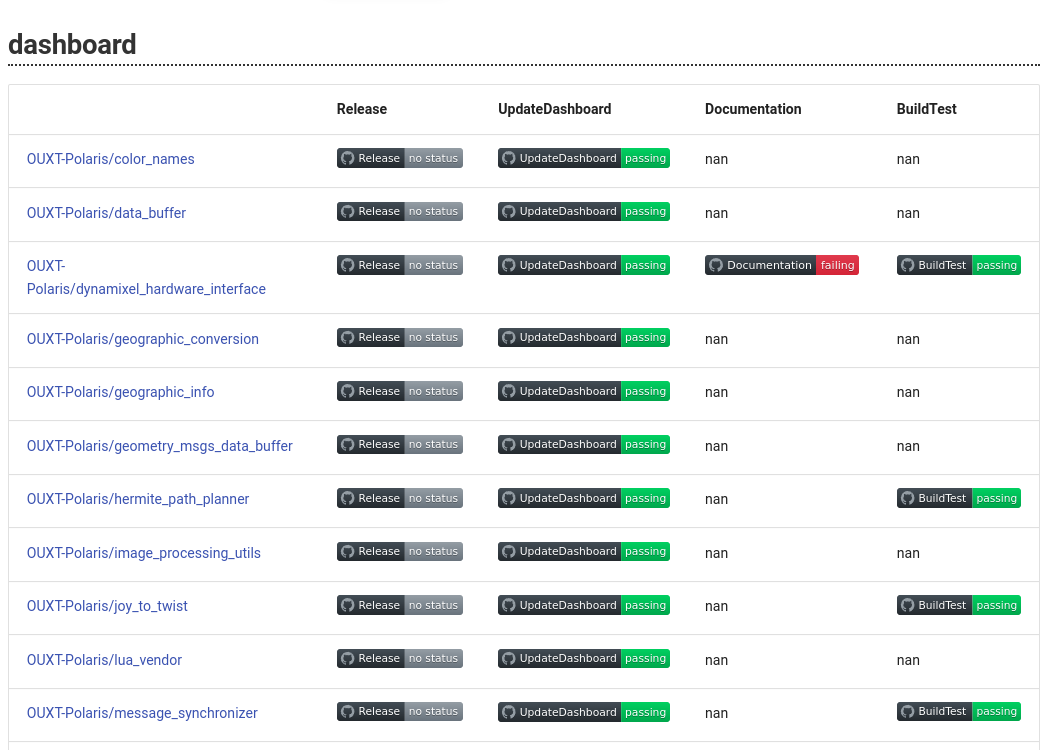
\includegraphics{figure/dashboard.png}
    }
  \end{center}
  \caption{CI/CD Dashboard}
  \label{fig:ci_cd_dashboard}
\end{figure}

We divide our packages into smaller pieces in order to maintain the high degree of component nature of the packages we develop.
This reduces unnecessary build targets and greatly reduces CI time (tests that originally took 30 minutes or more are now only 3 minutes).
However, since there are more than 40 packages under our control alone,
it is impossible to keep track of their development and testing status without tools.
Therefore, we built a system that calls the API of GitHub and automatically creates a dashboard in Fig.\ref{fig:ci_cd_dashboard}.
All of these deliverables are also open-source software.
We also developed GitHub Actions to configure GitHub Actions to unify CI procedures for multiple repositories and
built a system to synchronize CI procedures at all times via bot accounts. \cite{wam-v-tan_bot}

GitHub Actions is also used when deploying to the actual machine.
GitHub Actions has a function called Self-Hosted Runner, which allows you to remotely execute any command using your own computer.
Using this function, after the CI of the ROS2 package is completed, 
a configuration file with all commit hashes fixed is created and deployed to the actual device
using Github Actions/ansible based on that configuration file.
This allows our team to deploy the verified and up-to-date source code to the machine at the push of a button.
\subsection{A Mock Server}
We must report the vehicle's status as the Autonomous Maritime System heartbeat to a Technical Director server via a TCP connection. 
Our team usually tests navigation systems using a simulation environment, 
so we should check the heartbeat sentence on the simulation loop. 
To achieve it, we built a simple mock server. 
It displays received NMEA-like sentences from a simulation via a TCP connection.

\subsection{Controller}
The WAM-V control system adopted the ros2\_control\cite{ros2_control,wamv_control}.
The ros2\_control is a framework for real-time control of robots using ROS2.
The WAM-V control is are calculated as follows.
\begin{equation}
  M \dot\nu = -D(\nu)\nu + F_H(\nu) + \tau
  \label{eq:control_1}
\end{equation}


\section{Conclusion}
In this paper, OUXT-Polaris reported the development of the autonomous navigation system for the 2022 RobotX Challenge.
Based on the results of the 2018 RobotX Challenge, OUXT-Polaris rebuilt the system and
developed improved systems for the Maritime RobotX Challenge 2022.
We succeeded in constructing the highly reusable system by designing systems with high independence as parts,
in addition to high computing capacity and environmental recognition capability.
Moreover, we described the developing method in Covid-19 and the feature components for the next RobotX Challenge.
We hope these significant upgrades will produce positive results in the next competition.

% \section*{Acknowledgments}
\begin{thebibliography}{1}
\bibliographystyle{IEEEtran}
    \bibitem{robotx_ekf}
    \url{https://github.com/OUXT-Polaris/robotx_ekf}

    \bibitem{ROS2_paper}
    Steven Macenski, et al. "Robot Operating System 2: Design, architecture, and uses in the wild." Science Robotics (2022)

    \bibitem{ouxt_automation}
    \url{https://github.com/OUXT-Polaris/ouxt_automation.git}

    \bibitem{documentation_software}
    \url{https://ouxt-polaris.github.io/ouxt_automation/}

    \bibitem{documentation_hardware}
    \url{https://ouxt-polaris.github.io/robotx-hardware-documentation/}

    \bibitem{YOLOX}
    Ge, Zheng, et al. "Yolox: Exceeding yolo series in 2021." arXiv preprint arXiv:2107.08430 (2021).

    \bibitem{dataset_annotations}
    \url{https://github.com/OUXT-Polaris/dataset_annotations.git}

    \bibitem{RobotX2018_video}
    \url{https://www.youtube.com/watch?v=MqDBxzS4uy4}

    \bibitem{dataset_annotations}
    \url{https://github.com/OUXT-Polaris/scan_segmentation.git}

    \bibitem{wam-v-tan_bot}
    \url{https://github.com/wam-v-tan}

  \bibitem{ros2_control}
  \url{https://github.com/ros-controls/ros2_control}

  \bibitem{wamv_control}
  \url{https://github.com/OUXT-Polaris/wamv_control}

\end{thebibliography}

\vfill

\end{document}
